\documentclass[UTF8]{ctexart}
\title{简易Git指北}
\author{Gakusyun}
\date{\today}
\usepackage{times}
\usepackage{graphicx}
\usepackage{fancyhdr}
\usepackage{hyperref}
\hypersetup{hidelinks,
	colorlinks=true,
	allcolors=black,
	pdfstartview=Fit,
	breaklinks=true}
\usepackage[left=3.18cm, right=3.18cm, top=2.54cm, bottom=2.54cm]{geometry}
\pagestyle{fancy}  
\fancyhf{} % 清除默认页眉和页脚设置  
\fancyfoot[C]{\thepage} % 在页脚中央显示页码
\begin{document}
\maketitle
\thispagestyle{empty}
\newpage
\tableofcontents
\thispagestyle{empty}
\newpage
\section{前言}
本文旨在让同学0基础快速上手Git,不能作为Git的完整教程。
\newpage
\section{安装\ Git}
\subsection{Windows 环境}
\subsubsection{直接下载安装}
在官网 https://git-scm.com/ 下载安装包。如图\ref{install:downloadGit-Windows}所示。

然后在图\ref{install:gitinstaller}中点击下一步安装即可。
\begin{figure}[h]
    \centering
    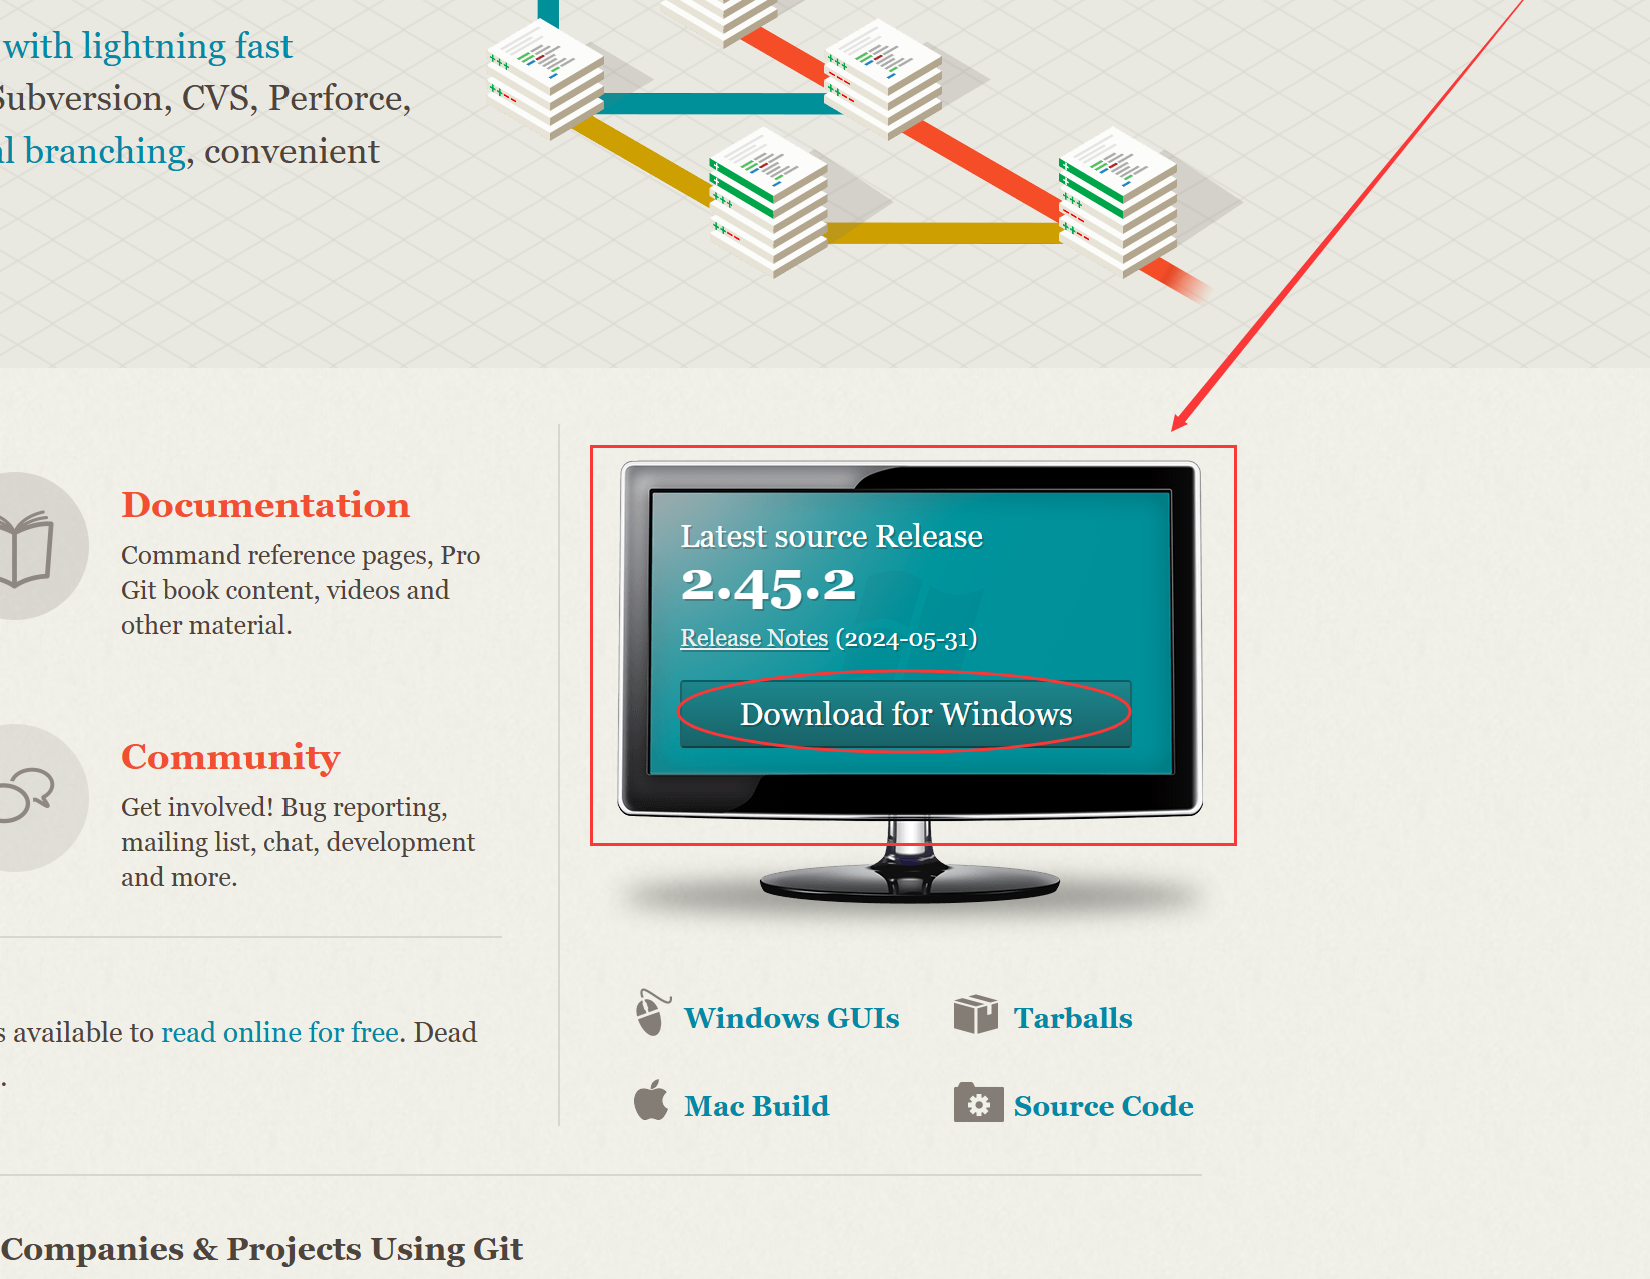
\includegraphics[width=0.6\textwidth]{./img/downloadGit-Windows}
    \caption{下载 Git 安装包}
    \label{install:downloadGit-Windows}
\end{figure}
\begin{figure}[h]
    \centering
    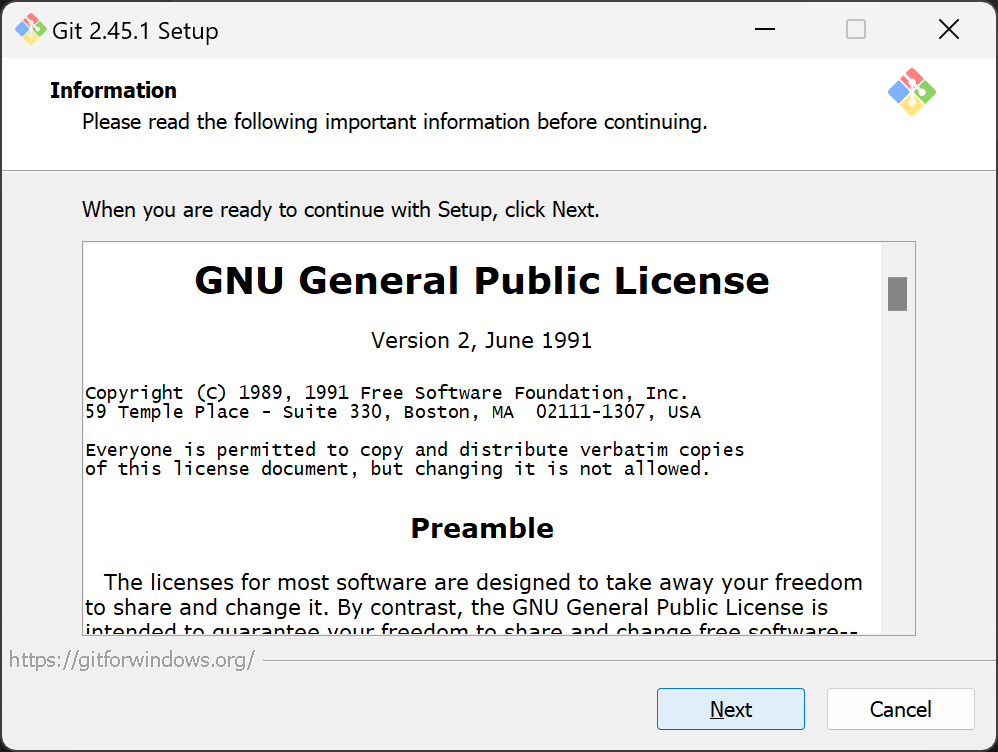
\includegraphics[width=0.6\textwidth]{./img/gitinstaller}
    \caption{安装 Git}
    \label{install:gitinstaller}
\end{figure}

\subsubsection{使用 Windows 下的包管理器安装}
\begin{enumerate}
    \item 使用Winget安装Git
          \begin{enumerate}
              \item 安装Winget:在Windows 10以上,Winget是默认安装的,这里不需要安装。
              \item 安装Git:在命令行中输入winget install Git.Git,即可安装Git。
          \end{enumerate}
    \item 使用Chocolatey安装Git
          \begin{enumerate}
              \item 安装Chocolatey:在官网 https://chocolatey.org/install 根据指引安装Chocolatey。
              \item 安装Git:在命令行中输入choco install git,即可安装Git。
          \end{enumerate}
    \item 使用Scoop安装Git
          \begin{enumerate}
              \item 安装Scoop:在官网 https://scoop.sh/ 根据指引安装Scoop。
              \item 安装Git:在命令行中输入scoop install git,即可安装Git。
          \end{enumerate}
\end{enumerate}
\subsection{Linux 环境}


\subsubsection{Debian/Ubuntu/Deepin:}使用apt安装Git:
\begin{verbatim}
        $ sudo apt install git
\end{verbatim}
\subsubsection{CentOS/Fedora:}使用yum安装Git:
\begin{verbatim}
        $ sudo yum install git
\end{verbatim}
\subsubsection{Arch Linux:}使用pacman安装Git:
\begin{verbatim}
        $ sudo pacman -S git
\end{verbatim}

或者使用Aur包管理器安装Git:
\begin{verbatim}
        $ yay -Syu git #滚动更新
\end{verbatim}
\newpage
\section{Git 配置}
\subsection{配置用户信息}
这里配置用户名是为了在提交代码时,Git能识别你的身份。在后面注册Github或Gitee时,也请使用你配置的用户名,绑定你这里的邮箱。
\begin{verbatim}
    # 以我的邮箱和用户名为例,使用时请替换成自己的邮箱和用户名
    $ git config --global user.name 'Gakusyun' 
    $ git config --global user.email 'gaoxj040620@outlook.com'
\end{verbatim}
\subsection{进阶:ssh 配置}
参照 \href{https://help.gitee.com/base/account/SSH公钥设置}{https://help.gitee.com/base/account/SSH公钥设置}这里不过多赘述。
\section{Git使用}
\subsection{创建仓库}
在命令行中使用 cd 命令跳转至你想创建仓库的目录,然后如图\ref{creat-git-base}使用 git init 命令初始化仓库。然后使用 git add * 命令将所有文件添加至暂存区,最后使用 git commit -m '提交信息' 命令提交代码。
\begin{figure}[h]
    \centering
    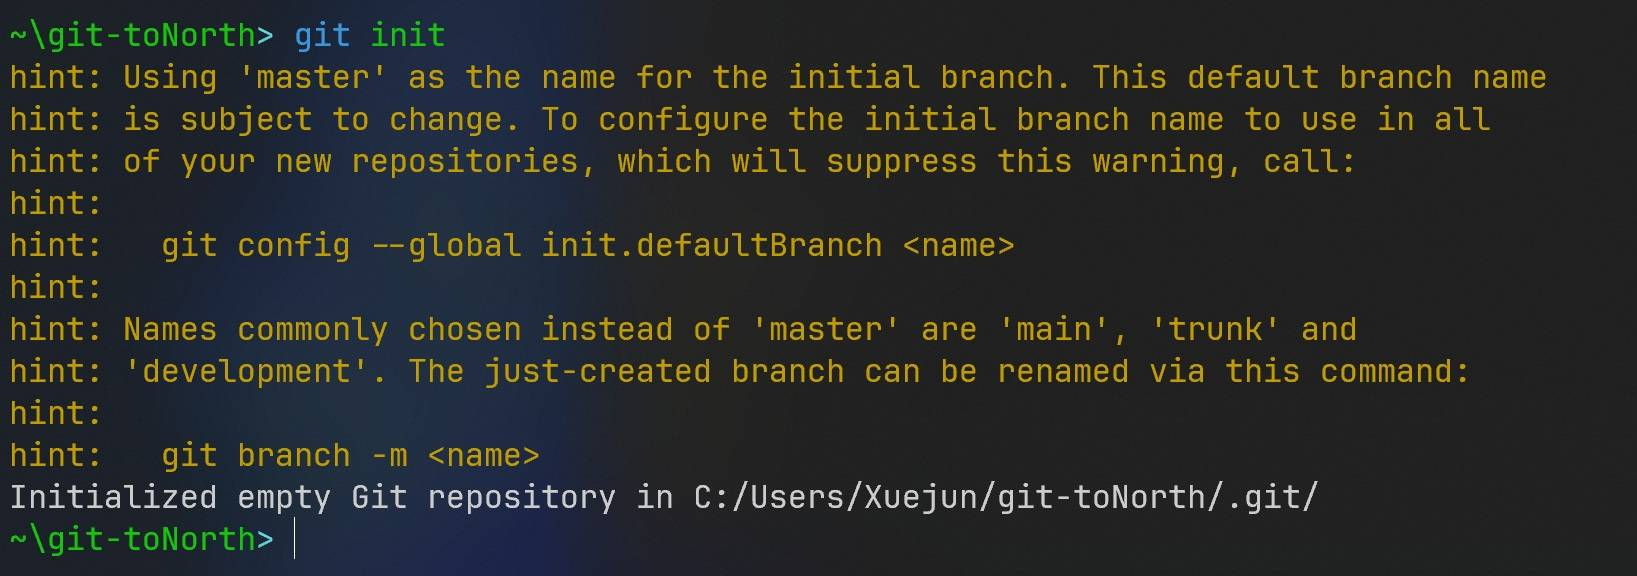
\includegraphics[width=0.8\textwidth]{./img/creat-git-base}
    \caption{创建仓库}
    \label{creat-git-base}
\end{figure}
这样,你就创建了一个仓库,并提交了第一次代码。
\begin{verbatim}
    $ cd /path/to/your/project
    $ git init
    $ git add *
    $ git commit -m 'first commit'
\end{verbatim}
\subsection{连接远程仓库}
在本地创建好仓库后,需要将本地仓库与远程仓库进行连接,才能和Teammates进行协作。这里使用,git remote add origin <EMAIL>:Gakusyun/one.git 命令将本地仓库与远程仓库进行连接。然后使用 git push -u origin master 命令将本地仓库推送到远程仓库。
\begin{verbatim}
    $ git remote add origin <EMAIL>:Gakusyun/one.git
    $ git push -u origin master
    # 第一次推送时,需要输入用户名和密码
    Username for 'https://gitee.com': username
    Password for 'https://username@gitee.com': password
    # 以后推送时,就不用输入用户名和密码了
    $ git push
\end{verbatim}
\subsection{推送本地仓库}
当你修改了代码后,使用 git add * 命令将所有文件添加至暂存区,然后使用 git commit -m '提交信息' 命令提交代码到本地仓库。提交后,使用 git push 命令将本地仓库推送到远程仓库.
\begin{verbatim}
    $ git add *
    $ git commit -m '提交信息'
    $ git push
\end{verbatim}
\subsection{拉取远程仓库}
当Teammates修改了远程仓库中的代码,你需要使用 git pull 命令将远程仓库的代码拉取到本地。
\begin{verbatim}
    $ git pull
\end{verbatim}
\section{结语}
本文的编译日期为\today,如果对本文有任何建议或意见,欢迎在本文的GitHub页面\href{http://github.com/Gakusyun/git-toNorth}{github.com/Gakusyun/git-toNorth}发表你的意见,或者参与对本文的修订。
\end{document}